% $Author: Luc $
% $Date: 2008-11-09 11:14:31 +0200 (Sun, 09 Nov 2008) $
% $Revision:  $
%=================================================================
\ifx\wholebook\relax\else
% --------------------------------------------
% Lulu:
    \documentclass[a4paper,10pt,twoside]{book}
    \usepackage[
        papersize={6in,9in},
        hmargin={.75in,.75in},
        vmargin={.75in,1in},
        ignoreheadfoot
    ]{geometry}
    \input{../common.tex}
    \pagestyle{headings}
    \setboolean{lulu}{true}
% --------------------------------------------
% A4:
%   \documentclass[a4paper,11pt,twoside]{book}
%   \input{../common.tex}
%   \usepackage{a4wide}
% --------------------------------------------
    \graphicspath{{figures/} {../figures/}}
    \begin{document}
%   \renewcommand{\nnbb}[2]{} % Disable editorial comments
    \sloppy
\fi

\chapter{Loops and Variables}\label{cha:loopsandvariables}

\noindent\hrule
\includegraphics[width=0.9\linewidth]{c5spiral91}
\noindent\hrule\vspace{1.5cm}

In this chapter I will show you how to use variables and loops in combination. We will begin 
by analyzing a simple problem that illustrates the need for using variables with loops. Then 
you will experiment with some other problems. 

\newpage
\section{A Bizarre Staircase}

Try to program a robot to draw the strange Staircase shown in Figure~\ref{fig:c5escaliertordu}. All of the risers have the same height, but the treads get longer and longer as you climb the staircase. One 
way to start is to write a script for a normal stairway and then modify it. You will need to solve 
the problem of making each tread longer than the previous one.


\begin{figure}[h!]
\center{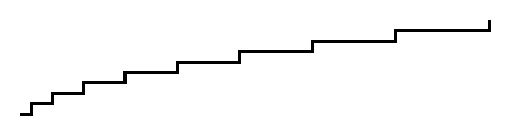
\includegraphics[width=10cm]{varLoopsFlatStair}}
\caption{Pica draws a bizarre staircase.\label{fig:c5escaliertordu}}
\end{figure}

A simple solution is shown in Script~\ref{scr:bizarrestaircase}, where the length of each tread grows by 10 pixels. However, such a solution is not satisfactory for two reasons: First, you have to compute 
the length of each tread manually. And second, you have to repeat an almost identical 
sequence of message sends over and over. 


\begin{script}[bizarrestaircase]{Pica draws the bizarre staircase.}
| pica | 
pica := Bot new. 
pica go: 10. 
pica turnLeft: 90. 
pica go: 5. 
pica turnRight: 90. 
pica go: 20. 
pica turnLeft: 90. 
pica go: 5. 
pica turnRight: 90. 
pica go: 30. 
pica turnLeft: 90. 
pica go: 5. 
pica turnRight: 90. 
pica go: 40. 
pica turnLeft: 90. 
pica go: 5. 
pica turnRight: 90. 
... 
\end{script}


We would like to be able to use the power of variables (to automate the increasing tread 
length) combined with the power of loops (so that we don’t have to type so much code). To 
avoid repeating the sequence of message sends you can use the \ct{timesRepeat:} message. And as 
for using variables, the key is to be found in an examination of Script~\ref{scr:bizarrestaircase}, where you will see 
that the length of each tread after the first is the length of the previous tread plus 10 pixels. 
After all, 20 = 10 + 10, 30 = 20 + 10, 40 = 30 + 10, and so on, as shown in Figure~\ref{fig:escalierexplications}. 

\begin{figure}[h!]
\center{\includegraphics[width=10cm]{stairExplained2}}
\caption{The length of a tread is the length of the previous tread plus 10 pixels.\label{fig:escalierexplications}}
\end{figure}

Let us use the variable \ct{treadLength} to represent the length of a tread. Then, once 
\ct{treadLength} has been initialized to the length of the first tread, the expression 
\ct{treadLength := treadLength + 10} will set the length of the \emph{next} tread to be the value of the \emph{current} tread increased by 10. The result is that if \ct{treadLength} is initialized to 10, and the first tread is drawn, that tread will of course have length 10. Then, after the expression \ct{treadLength := treadLength + 10} is executed, the next time a tread is drawn it will have length 20. And after 
the expression is executed again, the next tread will have length 30, and so on. 

Let’s combine everything! We will start with the script of a normal staircase (Script~\ref{scr:stairwaynormalsteps}). Then, in Script~\ref{scr:stairwaywithvar}, we obtain the same staircase, but using the variable \ct{treadLength}. Then in Script~\ref{scr:stairwayincrease}, we add the line \ct{treadLength := treadLength + 10} to change the \ct{treadLength} value in each step of the loop, and thus we finally obtain the stairway we want. 



\begin{script}[stairwaynormalsteps]{A stairway with normal steps.}
| pica | 
pica := Bot new. 
10 timesRepeat: 
	[ pica go: 10. 
	pica turnLeft: 90. 
	pica go: 5. 
	pica turnRight: 90 ] 
\end{script}


\begin{script}[stairwaywithvar]{A stairway with normal steps using the variable \ct{treadLength}.}
| pica !\textbf{treadLength}!| 
pica := Bot new. 
!\textbf{treadLength} := 10. !
10 timesRepeat: 
	[ pica go: !\textbf{treadLength}!. 
	pica turnLeft: 90. 
	pica go: 5. 
	pica turnRight: 90 ]
\end{script}

\begin{script}[stairwayincrease]{The solution: increasing the variable \ct{treadLength} each time through the loop produces the bizarre staircase.}
| pica !\textbf{treadLength}!| 
pica := Bot new. 
!\textbf{treadLength} := 10. !
10 timesRepeat: 
	[ pica go: !\textbf{treadLength}!. 
	pica turnLeft: 90. 
	pica go: 5. 
	pica turnRight: 90. 
	!\textbf{treadLength := treadLength + 10}!] 
\end{script}

Let’s look more closely at the sequence of expressions in the loop in Script~\ref{scr:stairwayincrease}. The first expression draws a tread by making the robot go forward a distance given by the value of the 
variable \ct{treadLength} (which has been initialized to \ct{10} for the first time through the loop). 
Then the robot turns, draws a riser (straight up), and turns again. Then the value of the variable \ct{treadLength} is increased by 10 and the loop restarts, but now the variable \ct{treadLength} 
has a new, larger, value (20 for the second repetition). The whole process is executed 10 times.

The expression \ct{treadLength := treadLength + 10} is absolutely necessary. Without it, the 
value of the variable would never change. 

\begin{exonofigtitle}{Placement of the Increment in the Loop}
Try changing the last line of the loop; for example, \ct{treadLength := treadLength + 15}. Then try moving the line to different places in the loop. Can you explain what happens when you move the last line of the loop to the beginning of the loop? 
\end{exonofigtitle}

If you are still uncertain about what is going on in Script~\ref{scr:stairwayincrease}, I suggest that you think carefully about the value of the variable \ct{treadLength}, especially at the beginning and end of 
the loop. Figure out the value of \ct{treadLength} in each expression for three repetitions of the 
loop. If necessary, read Chapter~\ref{cha:variables} again.


\section{Practice with Loops and Variables: Mazes, Spirals, and More} % 

Let’s see how combining variables and loops can help you to solve some other problems.

\begin{exofigwithsizeandtitle}[0.6]{\includegraphics[width=5cm]{2dstrangestair}}{Another Bizarre Staircase}
Modify Script~\ref{scr:stairwayincrease} to produce the picture shown below, which represents a staircase in which both the treads and the risers grow in size.
\end{exofigwithsizeandtitle}

\begin{exofigwithsizeandtitle}[0.6]{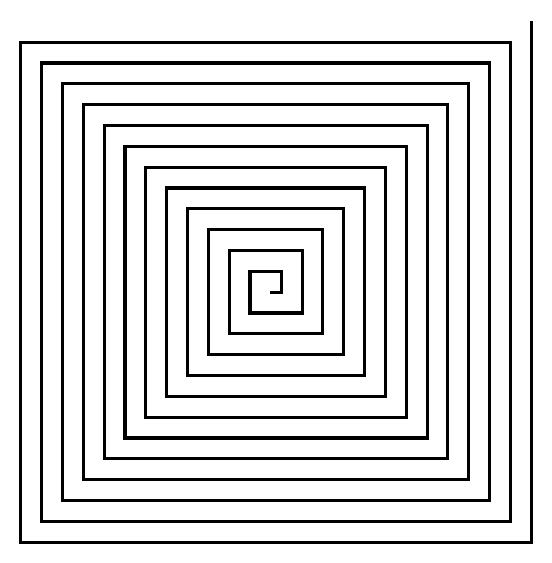
\includegraphics[width=5cm]{varLoopsMaze}}{A Simple Maze}
Write a script that reproduces the drawing shown below. In addition,by changing the angle through which the robot turns,you should be able to re-create the picture shown at the beginning of this chapter, as well as the spiral shown in Figure~\ref{fig:nicespiral}.
\end{exofigwithsizeandtitle}


\begin{figure}[h]
\center{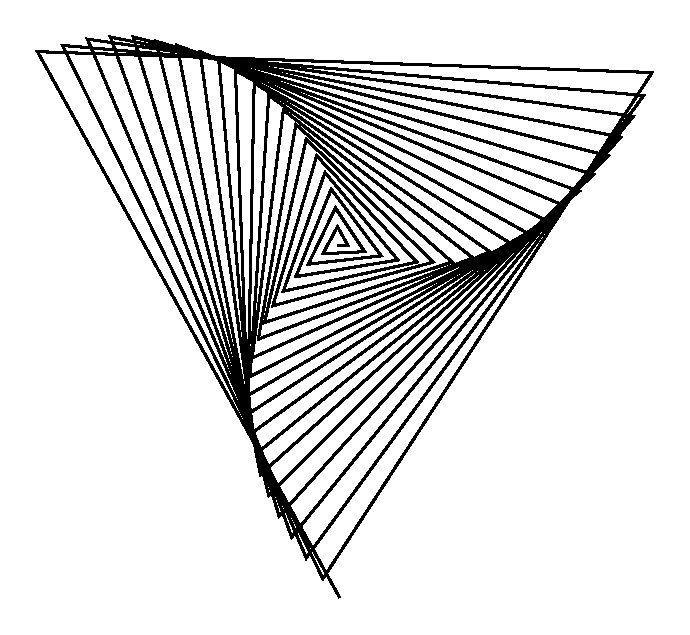
\includegraphics[width=10cm]{varLoopsSpiral121}}
\caption{A nice spiral.\label{fig:nicespiral}}
\end{figure}


\begin{exofigwithsizeandtitle}[0.6]{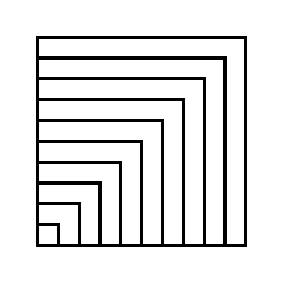
\includegraphics[width=5cm]{Argmirescr}}{Russian Squares}
Draw the nested squares of different sizes as shown in the figure below. You might begin by defining a loop that draws the same square ten times. Then introduce a variable \ct{sideLength} to represent the side length of a square, and finally,make the side length grow each time through your loop. As an additional challenge, you might try to write a new script that draws the same figure without the robot having either to jump or draw any line twice.	
\end{exofigwithsizeandtitle}


\begin{exofigwithsizeandtitle}[0.5]{\includegraphics[width=5cm]{corridor}}{A Long Corridor}
The concentric (having a common center) squares of different sizes shown in the figure below represent a long corridor, which seems to get smaller as you look into the distance. Again start by drawing a square, but this time draw it starting from its center (you will need a \ct{jump} message), so that when you change the square's size, the next square will automatically be drawn concentric to the first one. Now define your square inside a loop, and then introduce a variable \ct{sideLength} representing the side length of the square. Finally, make the square grow each time through your loop. 
\end{exofigwithsizeandtitle}


\section{Some Important Points for Using Variables and Loops}

Now that you have seen the overall process of combining loops and variables and have experimented a bit, I would like to stress some important points. Script~\ref{scr:variableinloop} shows a typical situation in outline form: First a variable is declared. Then it is initialized. Inside the loop, the variable is used to perform some computations, and then its value is changed for the next pass through the loop. 

\begin{script}[variableinloop]{An outline script showing the use of a variable in a loop.}
| treadLengthpica |                "variable declaration" 
...   
treadLength := 10.                  "initialization of the variable" 
...  
10 timesRepeat:  
[ pica go: treadLength.        "variable use" 
...  
treadLength := treadLength + 10]   "variable change of value" 
\end{script}


\section{Variable Initialization} 

When you introduce a variable in a loop, you have to pay special attention to the first value of 
the variable, that is, the value assigned to the variable when it is initialized. Keep in mind that 
a variable cannot be used until it has been initialized. Normally, variable initialization is done 
outside of the loop, for otherwise, the variable’s value would be reinitialized at each step of the 
loop, with the result that the value of the variable would not change. 

\section{Using and Changing the Value of a Variable}

Inside the loop, the variable’s value is often used to perform a variety of computations, such as to compute the values of other variables or perhaps to tell a robot how far to travel. Then the value of the variable is eventually changed. In the stairway example, the expression \ct{treadLength := treadLength + 10} increases the value of the tread length based on its preceding value. What is important to understand is that the new value assigned to the variable will be its value for the next step of the loop, as illustrated in Figure~\ref{fig:steppingLoop}. 

\begin{figure}
\center{\includegraphics[width=0.9\linewidth]{steppingLoop}}
\caption{The length of a tread is the length of the previous tread plus 10 pixels. The last value that a variable has in the loop body is the value that the variable will have at the start of the loop when it is repeated.\label{fig:steppingLoop}}
\end{figure}


\section{Advanced Experiments}

\begin{exofigwithsizeandtitle}[0.5]{\includegraphics[width=5cm]{damier}}{Squares}\label{xp:squares}
Define a script that creates the checkerboard construction shown below. This experiment is a bit more complicated than the earlier experiments, in that it is difficult to see how to draw the figure using a single loop. However, there are several ways of solving the problem using two loops. For example, you could use one loop to draw all the horizontal lines, and then another loop to draw all the vertical lines.	
\end{exofigwithsizeandtitle}

\begin{exofigwithsizeandtitle}[0.5]{\includegraphics[width=5cm]{cubesandpyramid}}{Pyramid}
Write a script that creates the construction shown in the figure below,representing the blocks of stones forming part of the step pyramid of Saqqara, which you have seen in previous chapters. You might modify your script from Experiment~\ref{xp:squares} by changing the variable for the length of the lines drawn each time through the loop. 
\end{exofigwithsizeandtitle}

\section{Summary}

\begin{itemize}
	\item When introducing a variable inside a loop, be careful how you initialize the variable. 
Keep in mind that a variable must be initialized before its value is used. Normally, initialization occurs outside the loop, for otherwise, the value of the variable would not change when the loop is repeated. 
\item Keep in mind that the last value that a variable is assigned in a loop body will be the 
variable’s value the next time the loop is executed.
\end{itemize}


\ifx\wholebook\relax\else
    \end{document}
\fi

%%% Local Variables:
%%% coding: utf-8
%%% mode: latex
%%% TeX-master: t
%%% TeX-PDF-mode: t
%%% ispell-local-dictionary: "english"
%%% End: